\label{Chapter1}

\section{Μεθοδολογία ανάπτυξης εφαρμογής}

\subsection{Διαθέσιμες μεθοδολογίες}

\subsubsection{Μοντέλο build and fix}

Το \textbf{μοντέλο build and fix} είναι ένα μοντέλο στο οποίο το λογισμικό έχει 
αναπτυχθεί χωρίς σχεδιασμό. Ουσιαστικά, κατασκευάζεται ένα αρχικό προϊόν και τροποποιείτε
μέχρι να ικανοποιήσει τον χρήστη. Το μοντέλο έχει δύο φάσεις:

\begin{itemize}
    \item Η φάση του \textbf{build}: Όπου ο κώδικας κατασκευάζεται
    και περνάει στην επόμενη φάση.
    \item Η φάση του \textbf{fix}: Όπου ο κώδικας έχει φτάσει σε bug και 
    error free στάδιο και μπορεί να παρουσιαστεί στον χρήστη και να τροποποιηθεί 
    κατάλληλα για να ικανοποιήσει τον τελικό χρήστη. 
\end{itemize}

\begin{center}
    \begin{tabular}{| p{8cm} | p{8cm} |}
        \hline
        \multicolumn{2}{|c|}{\textbf{Πλεονεκτήματα και Μειονεκτήματα του μοντέλου build and fix}} \\
        \hline
        \textbf{Πλεονεκτήματα} & \textbf{Μειονεκτήματα} \\
        \hline
        Χρειάζεται λιγότερη εμπειρία σε οποιονδήποτε άλλο τομέα εκτός του προγραμματισμού & Δεν υπάρχει ένας μετρητής στον οποίο κρίνετε ούτε η πρόοδος, ούτε η ποιότητα του προϊόντος και ούτε ο ρίσκο \\
        \hline
        Πολύ ταιριαστό για μικρά λογισμικά &  Ο κόστος είναι πελώριος επειδή χρειάζεται να γίνονται πάρα πολλές στο λογισμικό μέχρι να ικανοποιήσει τον τελικό χρήστη \\
        \hline
        Χρειάζεται λιγότερο πλάνο & Είναι πολύ ανεπίσημος τρόπος σχεδίασης ενός λογισμικού \\
        \hline
        & Η συντήρηση τέτοιων μοντέλων είναι δύσκολη \\
        \hline
    \end{tabular}
\end{center}

\subsubsection{Μοντέλο καταρράκτη}

Το \textbf{μοντέλο του καταρράκτη (waterfall model)} είναι ένα από τα πιο κλασσικά παραδείγματα του life cycle. Η ανάπτυξη του λογισμικού είναι γραμμική και πάει από βήμα σε βήμα, η οποία πηγαίνει από βήμα σε βήμα με την ίδια ακριβώς δουλεία, χωρίς να υπάρχει δυνατότητα να μπορεί να γυρίσει πίσω. Κάθε βήμα έχει ξεχωριστό στόχο.

\begin{center}
    \begin{tabular}{| p{7cm} | p{2cm} | p{6.5cm} |}
        \hline
        \multicolumn{3}{|c|}{\textbf{Τα βήματα του μοντέλου καταρράκτη}} \\
        \hline
        \textbf{Είσοδος στο βήμα} & \textbf{Βήμα} & \textbf{Έξοδος του Βήματος} \\
        \hline
        Οι απαιτήσεις του λογισμικού πραγματοποιείται μέσω επικοινωνίας & Ανάλυσης &  Οι προδιαγραφές του λογισμικού είναι ορισμένες \\
        \hline
        Οι προδιαγραφές του λογισμικού είναι ορισμένες & Σχεδίασης & Σχεδιασμός του εγγράφου προδιαγραφών \\
        \hline
        Σχεδιασμός του εγγράφου προδιαγραφών & Ανάπτυξη & Δημιουργία εκτέλεσης προϊόντος \\
        \hline
        Δημιουργία εκτέλεσης προϊόντος & Δοκιμή & Έτοιμο προϊόν \\
        \hline
        Έτοιμο προϊόν & Υλοποίηση & Παραδοτέο λογισμικό \\
        \hline
        Παραδοτέο λογισμικό & Συντήρησης & Αλλαγές στις προδιαγραφές \\
        \hline
    \end{tabular}
\end{center}

Το μοντέλο του καταρράκτη φαίνεται και παρουαστικά στο Σχήμα~\ref{fig:waterfall}. Υπάρχουν αρκέτες παραλλαγές του μοντέλου καταρράκτη, όπως το παράλληλο μοντέλο
όπου αρκετά βήματα γίνονται παράλληλα. Για αρκέτες περιπτώσεις είναι αρκέτα ταιριαστό μοντέλο, αφού έχει χρησιμοποιήθει πάρα πολλές φορές και είναι σίγουρο ότι δουλεύει.
Για αυτό τον λόγο, αρκέτες από τις μεθοδολογίες που το ακολούθησαν βαδίζουν στην ίδια λογική.

\begin{figure}[th]
    \centering
    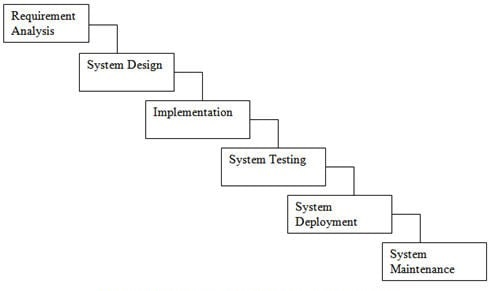
\includegraphics{Figures/waterfall.jpg}
    \caption[Το μοντέλο του καταρράκτη]{Το μοντέλο του καταρράκτη}
    \label{fig:waterfall}
\end{figure}

\newpage
\begin{center}
    \begin{tabular}{| p{8cm} | p{8cm} |}
        \hline
        \multicolumn{2}{|c|}{\textbf{Πλεονεκτήματα και Μειονεκτήματα του μοντέλου καταρράκτη}} \\
        \hline
        \textbf{Πλεονεκτήματα} & \textbf{Μειονεκτήματα} \\
        \hline
        Αρκετά απλό στην κατανόηση & Χρειάζεται να είναι οι προδιαγραφές έτοιμες πριν ξεκινήσει η ανάπτυξη \\
        \hline
        Κάθε βήμα της ανάπτυξης συνεχίζει διαδοχικά & Δεν μπορούν να γίνουν αλλαγές στις προδιαγραφές σε μεταγενέστερα βήματα του μοντέλου. Αυτό σημαίνει ότι ένα λογισμικό μπορεί να μπει στο στάδιο της δοκιμής θα είναι πολύ δύσκολο να γίνουν οι απαραίτητες αλλαγές \\
        \hline
        Επιτρέπει ελέγχο στην δημιουργία ενός προγράμματος με προθεσμίες σε κάθε βήμα & Δεν υπάρχει καμία επικοινωνία με τον τελικό χρηστή όσο το λογισμικό αναπτύσσετε \\
        \hline
        Βοηθάει στον έλεγχο των χρονοπρογράμματων, των προϋπολογισμών  και του εγγράφου & Δεν παίρνει υπόψιν του τον ρίσκο της διοίκησης \\
        \hline
        & Θεωρεί ότι οι προδιαγραφές είναι σταθερές και δεν αλλάζουν κατά την διάρκεια του κύκλου ζωής  \\
        \hline
    \end{tabular}
\end{center}

Μια δεύτερη παραλλαγή του μοντέλου καταρράκτη είναι το \textbf{μοντέλο της σπείρας (spiral model)}, το οποίο φαίνεται παρουσιαστικά στο Σχήμα~\ref{fig:spiral}.

\begin{center}
    \begin{tabular}{| p{8cm} | p{8cm} |}
        \hline
        \multicolumn{2}{|c|}{\textbf{Πλεονεκτήματα και Μειονεκτήματα του μοντέλου της σπειράς}} \\
        \hline
        \textbf{Πλεονεκτήματα} & \textbf{Μειονεκτήματα} \\
        \hline
        Παρέχει ένα εργατικό μοντέλο στον χρήστη νωρίς στην διεργασία και επιτρέπει μία πρόωρη εκτίμηση και αυξάνει την αυτοπεποίθηση του χρήστη & Άμα ο χρήστης δεν είναι ικανοποιημένος με το τελικό πρωτότυπο, τότε ένα νέο πρωτότυπο κατασκευάζεται. Έτσι επιτρέπει να δημιουργηθεί το τέλειο πρωτότυπο \\
        \hline
        Ο developer αποκτάει εμπειρίες και γνώση από την δημιουργία του πρωτότυπου και έτσι καταφέρνει να δημιουργήσει καλύτερες προδιαγραφές για την υλοποίηση & Ο developer χάνει το σωστό επίκεντρο του πρωτότυπου και έτσι χάνετε η ποιότητα της εφαρμογής \\
        \hline
        Το μοντέλο του πρωτότυπου πρέπει να εξυπηρετεί τις ανάγκες των προδιαγραφών οι οποίες δεν είναι καθαρές και έτσι μειώνει την ασάφεια και βελτιώνει την επικοινωνία μεταξύ των developers και των χρηστών & Τα πρωτότυπα μπορούν να οδηγήσουν σε λανθασμένες προσδοκίες \\
        \hline
        Βοηθάει στην μείωση των ρίσκων τα οποία συνδέονται με το λογισμικό & Ο κύριος στόχος είναι να γίνονται γρήγορα η ανάπτυξη και έτσι το παρακάτω μοντέλο είναι αρκετά αργό \\
        \hline
    \end{tabular}
\end{center}

\begin{figure}[th]
    \centering
    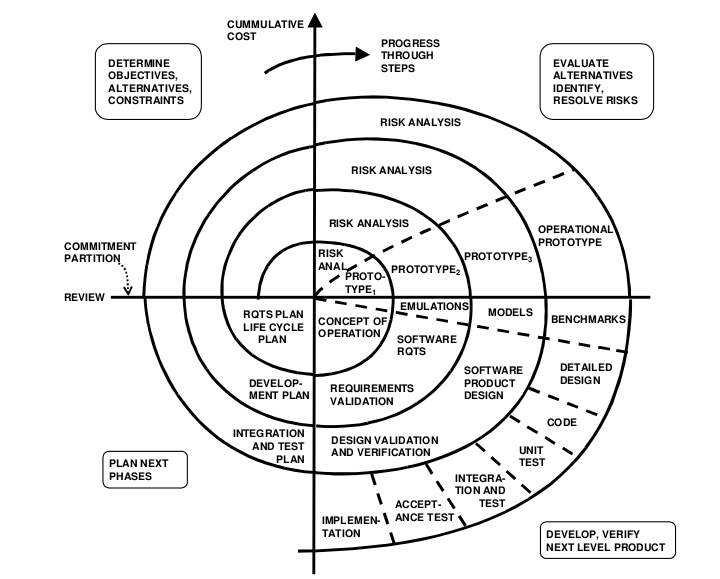
\includegraphics[width=150mm]{Figures/spiral.png}
    \caption[Το μοντέλο της σπειράς]{Το μοντέλο της σπειράς}
    \label{fig:spiral}
\end{figure}

\newpage
\subsubsection{Εξελεκτικές (Ταχείας Ανάπτυξης) Μεθοδολογίες}

Το \textbf{μοντέλο εξελικτικής ή ταχείας ανάπτυξης (Rapid Application Development, RAD)} είναι ένα μοντέλο το οποίο στηρίζετε στο να σπάει το μεγάλο πρότζεκτ σε μικρότερα πρότζεκτ και να δημιουργεί διάφορα πρωτότυπα ώστε να μπορούν να διακριθούν τα προβλήματα που υπάρχουν και να διορθωθούν. Ένα μεγάλο χαρακτηριστικό των RAD μοντέλων είναι ότι γίνετε επαναχρησιμοποίηση του ίδιου κώδικα, διεργασιών, templates και εργαλείων.
Οι φάσεις του RAD είναι οι εξής:

\begin{itemize}
    \item Σχεδιασμού
    \item Πρωτοτύπων
    \item Επανάληψη των βημάτων της ανάλυσης και των πρωτοτύπων όπου χρειάζεται
    \item Ολοκλήρωση των πρωτοτύπων
    \item Υλοποίηση
\end{itemize}

Στο Σχήμα~\ref{fig:rad} φαίνεται παρουαστικά πως μία τέτοια μεθοδολογία πρέπει να εφαρμοστεί. Μερικές rad μεθοδολογίες είναι το Rapid Programming και το Throwaway Prototyping.

\newpage
\begin{center}
    \begin{tabular}{| p{8cm} | p{8cm} |}
        \hline
        \multicolumn{2}{|c|}{\textbf{Πλεονεκτήματα και Μειονεκτήματα των RAD}} \\
        \hline
        \textbf{Πλεονεκτήματα} & \textbf{Μειονεκτήματα} \\
        \hline
        Για τα παραδοτέα είναι πολύ εύκολο στο να μπορούν να μεταφερθούν σε πιο υψηλού επίπεδου αφηρημένου κώδικα & Είναι χρήσιμο μόνο για μεγάλα project \\
        \hline
        Παρέχει πολύ μεγάλη ευελιξία στον επανασχεδιασμό σε περίπτωση που θεωρείτε απαραίτητο & Τα RAD project αποτυγχάνουν όταν δεν υπάρχει η απαραίτητη δέσμευση από τους developers ή τους χρήστες όταν το λογισμικό τελείωσει στην ώρα του \\
        \hline
        Μείωση της ανάγκης εγγραφής νέου κώδικα λόγο της χρήσης γεννήτριας κώδικα και επαναχρησιμοποίηση ήδη υπάρχων κώδικα & Δεν είναι αποδεκτό σε περίπτωση μεγάλου κινδύνου τεχνικών προβλημάτων \\
        \hline
        Ενθαρρύνει τους χρήστες στο να συμμετέχουν στην ανάπτυξη του project & Τα ενδιαφέροντα των χρηστών και των developers τείνουν στο να διαφέρουν με αποτέλεσμα να μην μπορούν να πραγματοποιηθούν οι απαιτήσεις του project με την χρήση του RAD μοντέλου \\
        \hline
        Πιθανότητα να υπάρχουν ελαττωματικά προϊόντα λόγω των πρωτοτύπων & \\
        \hline
    \end{tabular}
\end{center}

\begin{figure}[th]
    \centering
    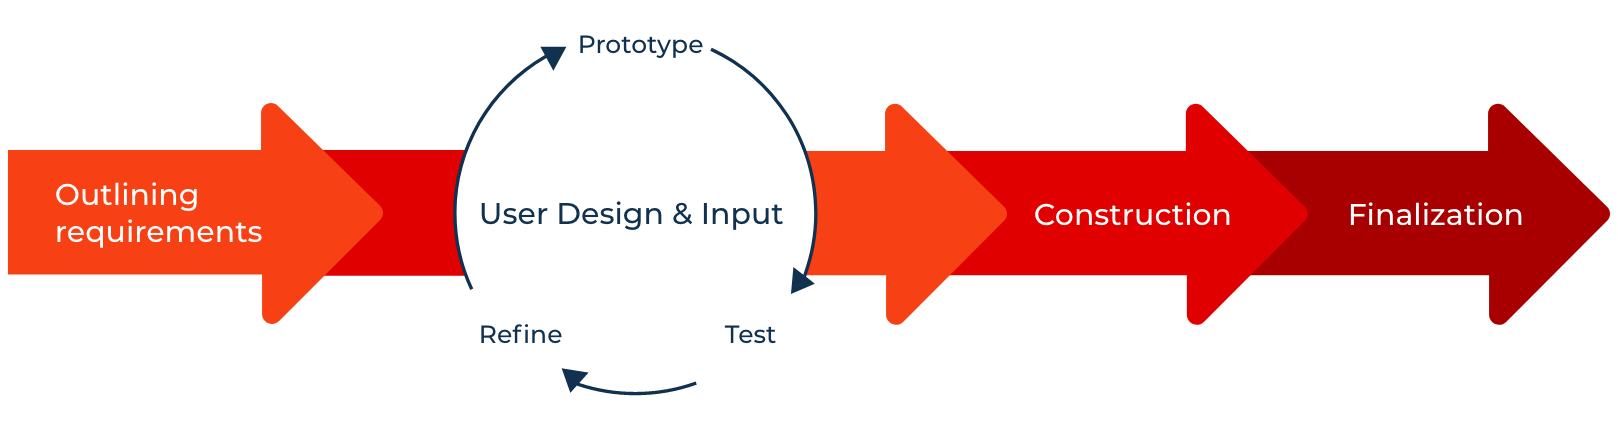
\includegraphics[width=150mm]{Figures/rad.png}
    \caption[Οι εξελικτές μεθοδολογίες]{Οι εξελικτές μεθοδολογίες}
    \label{fig:rad}
\end{figure}

\subsubsection{Εύκαμπτες/ευέλικτες μεθοδολογίες ανάπτυξης (Agile methodologies)}

Οι \textbf{εύκαμπτες μεθοδολογίες ανάπτυξης (Agile methodologies)} έχουν την ικανότητα να μπορούν να δημιουργούν και να αλληλεπιδρούν με την αλλαγή. 
Η διαφορά του Agile με άλλες μεθοδολογίες είναι ότι εστιάζει στους ανθρώπους της ομάδας και πως δουλεύουν μεταξύ τους. 
Οι λύσεις αναπτύσσονται μέσω συνεργασίας μεταξύ της αυτοδιοικούμενη ομάδα χρησιμοποιώντας πρακτικές για το context που βολεύει την κάθε ομάδα. 
Αυτό σημαίνει ότι δεν υπάρχουν διοικητές (managers) στην ομάδα, αλλά κάθε ομάδα έχει την ικανότητα να μπορεί να οργανωθεί μόνη της. 
Τα μέλη αυτής της ομάδας είναι ίσα και δεν έχουν συγκεκριμένους ρόλους μέσα στην ομάδα. 
To Agile, σύμφωνα με το Agile Manifesto έχει 12 βασικά θεμελιώδες ιδεολογίες:

\begin{enumerate}
    \item Η μεγαλύτερη προτεραιότητα είναι να ικανοποιηθεί ο πελάτης νωρίς και να υπάρχει συνέχει παράδοση καλού λογισμικού
    \item Να υπάρχουν αλλαγές στις προδιαγραφές μέχρι και όταν είναι αργά στο στάδιο της ανάπτυξης
    \item Να παραδίδετε ένα λειτουργικό λογισμικό συχνά, σε οποιονδήποτε χρονικό πεδίο
    \item Οι επιχειρηματίες και οι developers πρέπει να δουλεύουν μαζί καθημερινά κατά την διάρκεια όλου του project
    \item Να χτίζονται projects γύρο από άτομα που έχουν ισχυρό κίνητρο
    \item Η πιο αποτελεσματική μέθοδος στο να μπορεί να μεταφερθεί πληροφορία από και μέσω της developing ομάδας πρόσωπο προς πρόσωπο
    \item Ένα λειτουργικό λογισμικό είναι ο κύριος μετρητής της προόδου
    \item Οι διεργασίες της Agile προωθούν στο να μπορεί να υπάρξει ένα σταθερό development περιβάλλον από σπόνσορες, developers και χρήστες που θα μπορούν να συντηρήσουν μία σταθερή πρόοδο για μεγάλο χρονικό διάστημα
    \item Συνεχές προσοχή σε τεχνική τελειότητα και η καλή σχεδίαση βελτιώνει την Agile μεθοδολογία
    \item Η απλότητα και η τέχνη του περιορίζεται το μέγεθος της δουλείας που δεν γίνετε είναι ουσιώδες χαρακτηριστικό του Agile
    \item Οι καλύτερες αρχιτεκτονικές, προδιαγραφές και σχεδιάσεις έρχονται από αυτοδιοικούμενες ομάδες
    \item Σε συχνές συναντήσεις, η ομάδα ψάχνει πως μπορεί να γίνει όλο και πιο αποτελεσματική, κοιτάει τα λάθη της και συνεχίζει
\end{enumerate}

\begin{figure}[th]
    \centering
    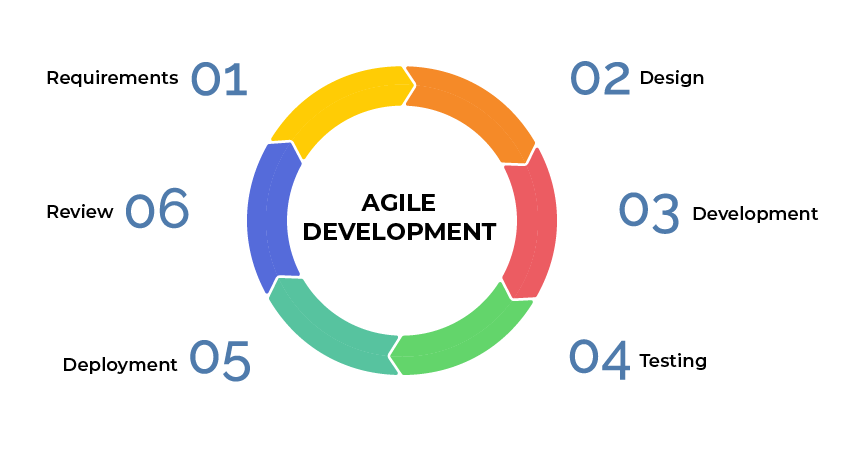
\includegraphics[width=150mm]{Figures/agile.png}
    \caption[Οι agile μεθοδολογίες]{Οι agile μεθοδολογίες}
    \label{fig:agile}
\end{figure}

Υπάρχουν αρκετές agile μεθοδολογίες, δύο από τις οποίες είναι το \textbf{extreme programming} και η \textbf{μεθοδολογία SCRUM}.

\subsection{Η Scrum μεθοδολογία}

To \textbf{Scrum} είναι ένα framework το οποίο βοηθάει τους ανθρώπους, τις ομάδες και τους οργανισμούς να δημιουργήσουν άξιες ευέλικτες λύσεις σε περίπλοκα προβλήματα. 
Το Scrum χρειάζεται έναν \textbf{Scrum Master} να καλλιεργεί το περιβάλλον όπου:

\begin{enumerate}
    \item Ένας πελάτης ζητάει δουλεία για την λύση του προβλήματος του σε ένα product backlog
    \item Η Scrum ομάδα επιλέγει ένα τμήμα της δουλείας που πρέπει να κάνει αναλόγως με την αξία της δουλείας σε ένα Sprint
    \item Η Scrum ομάδα και οι ενδιαφερόμενοι ελέγχουν τα αποτελέσματα τους και προσαρμόζονται για το επόμενο Sprint
    \item Επανάληψη της διαδικασίας
\end{enumerate}

Με λίγα λόγια, το Scrum ιδρύθηκε την κλίση προς τον εμπειρισμό και την λογική. 
\textbf{Εμπειρισμός} είναι η γνώση η οποία προέχεται από την εμπειρία και επιτρέπει στο να δημιουργήθουν αποφάσεις γύρο από αυτήν, ενώ \textbf{η λογική} ξεχωρίζει τις σημαντικές λεπτομέρειες του προϊόντος για να μπορεί να γίνει σωστή διαχείριση του χρόνου.
Το Scrum επιτρέπει ομάδες ανθρώπων να δουλέψουν μάζι και να μπορούν να αύξησουν την παραγωγικότητα και να προβλέψουν τον ρίσκο.
Τα τέσσερα στάδια του Scrum όνομαζονται Sprint, όπου γίνετε προσπάθεια να εφαρμοστούν οι αξίες του Scrum με διαφάνεια, έλεγχο και προσαρμογή.
Οι αξίες του Scrum είναι η δέσμευση, η συγκέντρωση, η ειλικρίνεια, ο σεβασμός και το κουράγιο.

\begin{figure}[th]
    \centering
    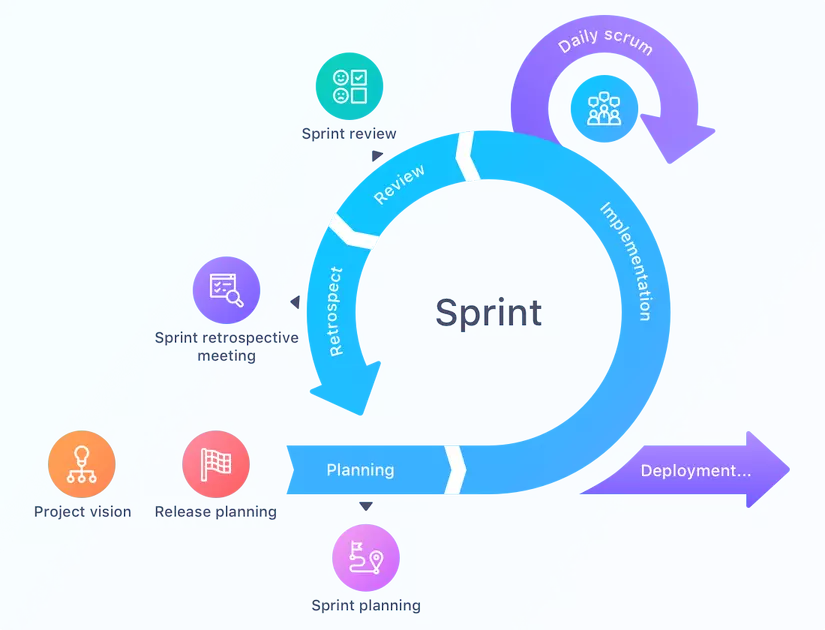
\includegraphics[width=150mm]{Figures/scrum.png}
    \caption[Το SCRUM μοντέλο]{Το SCRUM μοντέλο}
    \label{fig:scrum}
\end{figure}

\newpage
\subsection{Η Scrum ομάδα}
\subsubsection{Οι developers}

Οι \textbf{developers}, οι οποίοι είναι υπεύθυνοι να φτιάξουν κάθε μορφή ένος λειτουργικού σταδίου σε κάθε Sprint.
Οι ικανότητες που θα πρέπει να έχουν είναι:

\begin{itemize}
    \item Να μπορούν να δημιουργήσουν ένα σχέδιο για το Sprint, ονόματι \textbf{Sprint Backlog}
    \item Να μπορούν να κρατούν σταθερή την ποιότητα
    \item Να μπορούν μέρα με την μέρα να φτάσουν στον στόχο τους
    \item Να είναι όλοι ίσοι και σημαντικοί ως επαγγελματίες
\end{itemize}

\subsubsection{Ο ιδιοκτήτης του προϊόντος}

Ο \textbf{ιδιοκτήτης του προϊόντος (product owner)} συνήθως είναι ένας ανθρώπος και είναι υπεύθυνος να μπορεί να αυξήσει την αξία του προϊόντος του όσο πιο ψήλα γίνετε μέσα από την ομάδα του Scrum.
Επιπρόσθετα, είναι μπορεί και από επιλογή του να είναι υπεύθυνος ή να μεταφέρει την υπευθυνότητα του σε κάποιον αλλόν πάνω στην διαχείριση του backlog. Αυτές οι αρμοδιότητες είναι οι εξής:

\begin{itemize}
    \item Να μπορεί να μεταφέρει τον στόχο του προϊόντος
    \item Να δημιουργεί και να αφαιρεί τα στοιχεία του backlog που έχουν ολοκληρωθεί
    \item Να παραγγέλνει ότι αντικείμενο χρείαζεται
    \item Να επιβεβαιβεώνει ότι ύπαρχει διαφάνεια στο προϊόν όπως και να είναι κατανοήτο από όλους
\end{itemize}

Για να θεωρηθεί επιτυχημένος ο product owner, θα πρέπει να τον σέβονται όλοι στην ομάδα και στην εταίρεια. 

\subsubsection{Scrum Master}

Ο \textbf{Scrum master} είναι υπεύθυνος στο να ιδρύει το scrum όπως όριζεται από το Scrum Guide. 
Αυτό το πετυχένει βοηθόντας όλους να καταλάβουν το θεωρετικό και πρακτικό υπόβαθρο του Scrum και μέσα στην ομάδα και στον οργανισμό.
Με αλλά λόγια, ο Scrum Master είναι υπεύθυνος για το πόσο αποτελεσματική είναι η ομάδα και πολλές φόρες είναι αυτός που θα προσπαθήσει να λύσει τα υπαρχούσα προβλήματα. 

\subsection{Πλεονεκτήματα του scrum}

Ένα από τα βασικά πλεονεκτήματα της ευέλικτης μεθοδολογίας είναι η συνεχής ανάδραση σχολίων και κριτικής τόσο από τη μεριά του πελάτη όσο και από την μεριά της ομάδας σε κάθε κύκλο ανάπτυξης.
Αυτό έχει σαν αποτέλεσμα την ουσιαστικότερη κατανόηση των, πολλές φορές, μεταβαλλόμενων απαιτήσεων και λειτουργιών του project.
Επιπροσθέτως, ο πελάτης βλέποντας συχνά ένα παραδοτέο που συνεχώς παρατάσσεται μειώνεται το άγχος της απόσβεσης των χρημάτων που έχει καταβάλλει καθώς και η ενδεχομένως δυσπιστία και έλλειψη εμπιστοσύνης στην διαχείριση και της δυνατότητες της ομάδας.
Επίσης το συναίσθημα του ότι όλοι στην ομάδα ανάπτυξης είναι ιεραρχικά ίσοι και ότι όλοι έχουν εξίσου υποχρεώσεις και κοινές αρμοδιότητες, συνδράμει θετικά στην παραγωγικότητα και τη ψυχολογία της ομάδας καθώς και τους βοηθάει να κάνουν πρόοδο σε λιγότερες εργατοώρες.
Τέλος βασικό προτέρημα αποτελεί το γεγονός ότι λόγω των συνεχών συναντήσεων, η ομάδα είναι σε θέση να αντιμετωπίζει τα καθημερινά προβλήματα που προκύπτουν χωρίς να χρειάζεται να περιμένει μεγάλες περιόδους που ίσως να αποτελούν τροχοπέδη στην παραγωγικότητά και ευρυθμία της.

\subsection{Πιθανά ρισκά του scrum}

Το κύριο ρίσκό της μεθοδολογίας είναι ότι για να εφαρμοστεί απαιτεί ομάδα με εμπειρία έχει αυτοπειθαρχία και να μη παρασυρθεί από το συναίσθημα ελευθερίας που προσφέρει η πολιτική της συγκεκριμένης μεθοδολογίας καθώς και να είναι σε θέση να κρίνει αν πρέπει να γίνει η εναλλαγή σε κάποια άλλη μεθοδολογία αν αυτό κριθεί απαραίτητο σε ορισμένες φάσεις το έργου.
Θα ήταν παράβλεψη αν δεν  αναφερόταν το μειονέκτημα του να έχεις συχνές συναντήσεις με την ομάδα, αυτό μπορεί να αποδεχτεί δύσκολή και χρονοβόρα διαδικασία για ορισμένη μέλη της.
Συν του ότι αν κάποιος αρρωστήσει ή φύγει-παραιτηθεί οι σύντομες και ασφυκτικές προθεσμίες δεν θα μπορούν να ικανοποιηθούν και το έργο θα αρχίσει να αργεί ή ακόμη και να ακυρωθεί αν δεν βρεθούν αντικαταστάτες γρήγορα.  
Ακόμη, επειδή τα μέλη της ομάδας ασχολούνται με πολλές διεργασίες-δουλειές που πολλές φορές αλλάζουν προτεραιότητα αυτό οδηγεί σε  σύγχυση και καθυστέρηση της συνολικής προόδου της ομάδας.
